\chapter{Исследовательская часть}

В данном разделе приведены постановка эксперимента. 

\section{Формализация объекта и его признака}\label{formal}

Согласно согласованному варианту, формализуем объект <<блюда>> следующим образом: 
определим набор данных и признак объекта, на основании которого составим набор термом.

Набор данных для объекта:
\begin{itemize}
	\item название блюда --- строка;
	\item тип блюда --- строка;
	\item родина блюда --- строка.
\end{itemize}

Согласно варианту, числовым признаком, по которому будет производиться поиск объектов, является калорийность. 
Калорийность выражается количеством калорий на 100 грамм блюда --- вещественное число. 

Определим следующие термы, соответствующие признаку <<калорийность>>:
\begin{enumerate}
	\item очень не калорийное (сокр. ОН);
	\item не калорийное (сокр. Н);
	\item малой (сокр. М);
	\item средней (сокр. С);
	\item высокой(сокр. В);
	\item очень не высокой(сокр. ОНВ);
	\item не очень высокой (сокр. НОВ);
	\item <<не съем>>.
\end{enumerate}	

\clearpage

Также введем универсальное для задачи множество оцениваемой величины (калорийность) $K$:
\begin{equation}
	\label{eq:k}
	\begin{aligned}
	K = \{10, 20, 30, 40, 50, 100, 150, 200, 250, 300, 350, 400, 450, 500, 550, \\ 600, 650, 700, 750, 800, 850, 900, 950, 1000\}
	\end{aligned}
\end{equation}

\section{Анкетирование}

Было проведено анкетирование следующих респондентов:
\begin{enumerate}[label=\arabic*)]
	\item Назиров Илхом, группа ИУ7-55Б --- Респондент 1;
	\item Калашников Сергей, группа ИУ7-53Б --- Респондент 2;
	\item Лубянская Анастасия, группа ИУ7-56Б --- Респондент 3;
	\item Шагалов Вячеслав, группа ИУ7-51Б --- Респондент 4;
	\item Морозов Дмитрий, группа ИУ7-52Б --- Респондент 5;
	\item Нарандаев Дамир, группа ИУ7-52Б --- Респондент 6;
	\item Вязовцев Максим, группа ИУ7-55Б --- Респондент 7;
	\item Загайнов Никита, группа ИУ7-52Б --- Респондент 8.
\end{enumerate}

Респонденты, выступающие в качестве экспертов, для каждого из приведенных выше термов указали соответствующий промежуток, элементами которого являются числа из введенного для поставленной задачи множества оцениваемой величины.

Результаты анкетирования перечисленных респондентов продемонстрированы в таблицах~\ref{tbl:result_application_1} -- \ref{tbl:result_application_2}. В данных таблицах термы соответствуют обозначенным в \ref{formal} сокращенным термам.

\clearpage

\begin{table}[ht]
	\small
	\begin{center}
		\begin{threeparttable}
		\caption{Результаты анкетирования (Часть 1)}
		\label{tbl:result_application_1}
		\begin{tabular}{|c|c|c|c|c|c|c|}
			\hline
			\multirow{2}{*}{\bfseries Респондент} & \multicolumn{6}{c|}{\bfseries Терм, ккал/100 гр} \\ \cline{2-7}
			 & \bfseries ОН & \bfseries Н & \bfseries М & \bfseries С & \bfseries В & \bfseries не съем \\
			\hline
			1 & \text{[10; 30)} & \text{[30; 100)} & \text{[100; 300)} & \text{[300; 550)} & \text{[550; 850)} & >850 \\
			\hline
			2 & \text{[40; 100)} & \text{[10; 40)} & \text{[100; 400)} & \text{[400; 600]} & \text{[600; 1000)} & >1000 \\
			\hline
			3 & \text{[10; 100)} & \text{[100; 250)} & \text{[250; 350)} & \text{[350; 600]} & \text{[600; 1000]} & >1000 \\
			\hline
			4 & \text{10} & \text{20} & \text{(20; 150)} & \text{[150; 550)} & \text{[550; 1000)} & >1000 \\
			\hline
			5 & \text{10} & \text{(10; 40)} & \text{[40; 50)} & \text{[50; 150)} & \text{[150; 650)} & >650 \\
			\hline
			6 & \text{[10; 30)} & \text{[30; 50)} & \text{[50; 100)} & \text{[100; 200)} & \text{[200; 550)} & >550 \\
			\hline
			7 & \text{[10; 50)} & \text{[50; 200)} & \text{[200; 350)} & \text{[350; 550)} & \text{[500; 1000]} & >1000 \\
			\hline
			8 & \text{[10; 40)} & \text{[40; 150)} & \text{[150; 300)} & \text{[300; 450)} & \text{[450; 600)} & >600 \\
			\hline
		\end{tabular}
		\end{threeparttable}
	\end{center}
\end{table}

\begin{table}[ht]
	\small
	\begin{center}
		\begin{threeparttable}
			\caption{Результаты анкетирования (Часть 2)}
			\label{tbl:result_application_2}
			\begin{tabular}{|c|c|c|}
				\hline
				\multirow{2}{*}{\bfseries Респондент} & \multicolumn{2}{c|}{\bfseries Терм, ккал/100 гр} \\ \cline{2-3}
				& \bfseries ОНВ & \bfseries НOВ \\
				\hline
				1 & \text{[10; 150)} & \text{[150; 850)} \\
				\hline
				2 & \text{[10; 100)} & \text{[500; 700)} \\
				\hline
				3 & \text{[10; 350)} & \text{[350; 600)} \\
				\hline
				4 & \text{[10; 350)} & \text{[350; 600)}  \\
				\hline
				5 & \text{[10; 150)} & \text{[200; 400)} \\
				\hline
				6 & \text{[10; 100)} & \text{[350; 550)} \\
				\hline
				7 & \text{[10; 350)} & \text{[350; 600)} \\
				\hline
				8 & \text{[10; 100)} & \text{[100; 400)} \\
				\hline
			\end{tabular}
		\end{threeparttable}
	\end{center}
\end{table}

Результаты анкетирования перечисленных респондентов для каждого значения множества $K$ продемонстрированы в таблицах~\ref{tbl:tb_1} -- \ref{tbl:tb_2}. 
В данных таблицах термы соответствуют обозначенным в \ref{formal} сокращенным термам.
В ячейках таблицах хранятся количество респондентов указавший значение, которое будет соответствовать терму.

\clearpage

\begin{table}[ht]
	\small
	\begin{center}
		\begin{threeparttable}
			\caption{Результаты анкетирования по значениям множества $K$ (Часть 1)}
			\label{tbl:tb_1}
			\begin{tabular}{|c|c|c|c|c|c|c|c|c|c|c|c|c|c|c|}
				\hline
			    \multirow{2}{*}{\bfseries Терм} & \multicolumn{14}{c|}{\bfseries Калории, ккал/100 гр} \\ \cline{2-15}
				& 10 & 20 & 30 & 40 & 50 & 100 & 150 & 200 & 250 & 300 & 350 & 400 & 450 & 500 
				\csvreader{csv/research.csv}{}
				{\\\hline \csvcoli & \csvcolii & \csvcoliii & \csvcoliv & \csvcolv & \csvcolvi & \csvcolvii & \csvcolviii & \csvcolix & \csvcolx & \csvcolxi & \csvcolxii & \csvcolxiii & \csvcolxiv & \csvcolxv} \\
				\hline
			\end{tabular}
		\end{threeparttable}
	\end{center}
\end{table}


\begin{table}[ht]
	\small
	\begin{center}
		\begin{threeparttable}
			\caption{Результаты анкетирования по значениям множества $K$  (Часть~2)}
			\label{tbl:tb_2}
			\begin{tabular}{|c|c|c|c|c|c|c|c|c|c|c|c|}
				\hline				
				\multirow{2}{*}{\bfseries Терм} & \multicolumn{11}{c|}{\bfseries Калории, ккал/100 гр} \\ \cline{2-12}
				& 550 & 600 & 650 & 700 & 750 & 700 & 850 & 900 & 950 & 1000 & >1000
				\csvreader{csv/research.csv}{}
				{\\\hline \csvcoli &\csvcolxvi & \csvcolxvii & \csvcolxviii & \csvcolxix & \csvcolxx & \csvcolxxi & \csvcolxxii & \csvcolxxiii & \csvcolxxiv & \csvcolxxv & \csvcolxxvi} \\
				\hline
			\end{tabular}
		\end{threeparttable}
	\end{center}
\end{table}

\clearpage

\section{Построение функции принадлежности термам}

Для этого для каждого значения из $K$ для каждого терма из перечисленных найдем количество респондентов, согласно которым значение из $H$ удовлетворяет сопоставляемому терму.
Данное значение поделим на количество респондентов --- это и будет значением функции $m$ для терма в точке.
Графики функций принадлежности числовых значений калорийности термам, приведен на рисунке \ref{fig:graf}.

\begin{figure}[h]
	\centering
	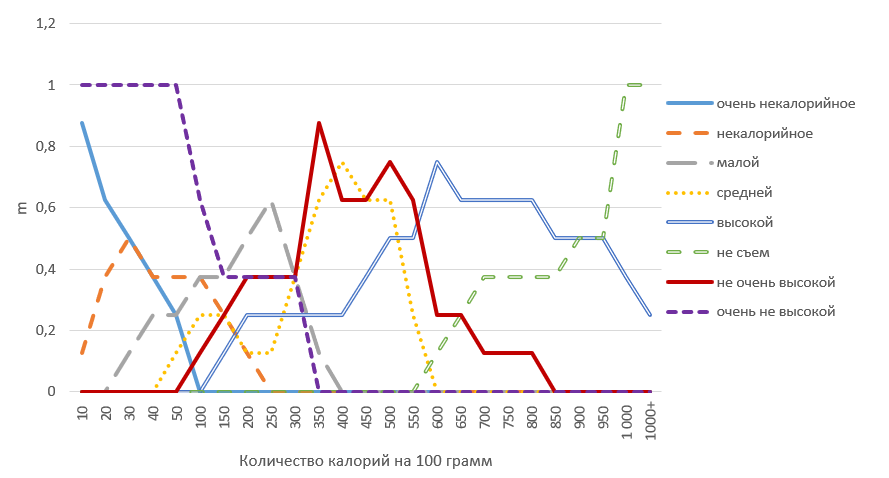
\includegraphics[width=0.9\textwidth]{img/graf.png}
	\caption{Графики функций принадлежности числовых значений переменной термам, описывающим группы значений лингвистической переменной}
	\label{fig:graf}
\end{figure}

В соответствии с полученным графиком будем считать блюда:
\begin{enumerate}
	\item очень некалорийной, если их значение их калорийность лежит в промежутке $[10; 25]$ калорий на 100 грамм;
	\item некалорийной, если их значение их калорийность лежит в промежутке $[26; 96]$ калорий на 100 грамм;
	\item малой калорийности, если их значение их калорийность лежит в промежутке $[96; 294]$ калорий на 100 грамм;
	\item средней калорийности, если их значение их калорийность лежит в промежутке $[295; 512]$ калорий на 100 грамм;
	\item высокой калорийности, если их значение их калорийность лежит в промежутке $[513; 954]$ калорий на 100 грамм;
	\item <<не съем>> калорийности, если их значение их калорийность больше 955 калорий на 100 грамм;
	\item очень не высокой калорийности, если их значение их калорийность лежит в промежутке $[10; 112]$ калорий на 100 грамм;
	\item не очень высокой калорийности, если их значение их калорийность лежит в промежутке $[263; 523]$ калорий на 100 грамм;
\end{enumerate}

\section{Тестирование}
В этом разделе представлены запросы пользователя и результаты их обработки.

\begin{figure}[h]
	\centering
	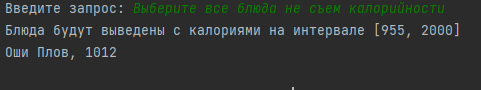
\includegraphics[width=0.9\textwidth]{img/request-1.png}
	\caption{Запрос 1}
	\label{fig:r1}
\end{figure}

\begin{figure}[h]
	\centering
	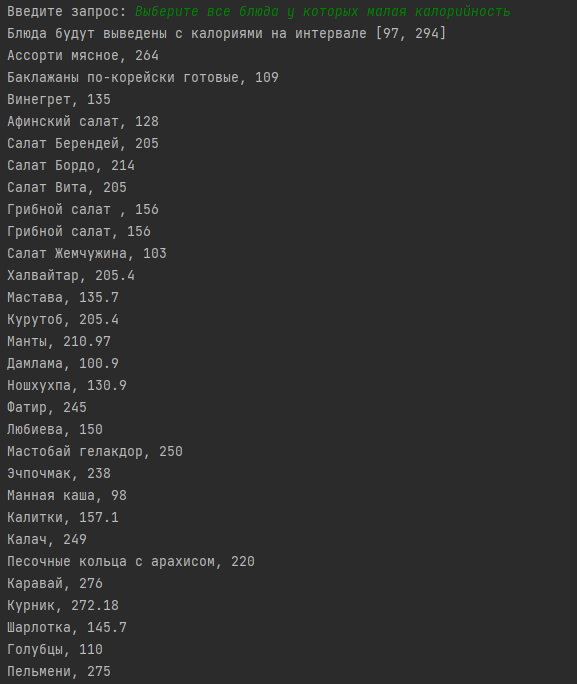
\includegraphics[width=0.9\textwidth]{img/request-2.png}
	\caption{Запрос 2}
	\label{fig:r2}
\end{figure}

\clearpage

\begin{figure}[h]
	\centering
	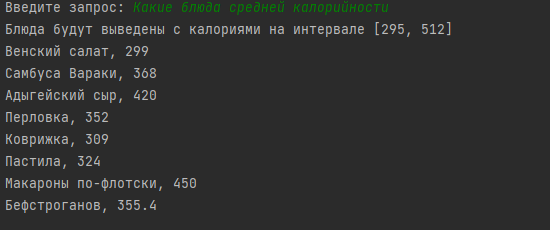
\includegraphics[width=0.9\textwidth]{img/request-3.png}
	\caption{Запрос 3}
	\label{fig:r3}
\end{figure}

\begin{figure}[h]
	\centering
	
\includegraphics[width=0.9\textwidth]{img/request-4.png}
	\caption{Запрос 4}
	\label{fig:r4}
\end{figure}

\begin{figure}[h]
	\centering
	
\includegraphics[width=0.9\textwidth]{img/request-5.png}
	\caption{Запрос 5}
	\label{fig:r5}
\end{figure}